\documentclass[twoside]{book}

% Packages required by doxygen
\usepackage{calc}
\usepackage{doxygen}
\usepackage{graphicx}
\usepackage[utf8]{inputenc}
\usepackage{makeidx}
\usepackage{multicol}
\usepackage{multirow}
\usepackage{textcomp}
\usepackage[table]{xcolor}

% Font selection
\usepackage[T1]{fontenc}
\usepackage{mathptmx}
\usepackage[scaled=.90]{helvet}
\usepackage{courier}
\usepackage{amssymb}
\usepackage{sectsty}
\renewcommand{\familydefault}{\sfdefault}
\allsectionsfont{%
  \fontseries{bc}\selectfont%
  \color{darkgray}%
}
\renewcommand{\DoxyLabelFont}{%
  \fontseries{bc}\selectfont%
  \color{darkgray}%
}

% Page & text layout
\usepackage{geometry}
\geometry{%
  a4paper,%
  top=2.5cm,%
  bottom=2.5cm,%
  left=2.5cm,%
  right=2.5cm%
}
\tolerance=750
\hfuzz=15pt
\hbadness=750
\setlength{\emergencystretch}{15pt}
\setlength{\parindent}{0cm}
\setlength{\parskip}{0.2cm}
\makeatletter
\renewcommand{\paragraph}{%
  \@startsection{paragraph}{4}{0ex}{-1.0ex}{1.0ex}{%
    \normalfont\normalsize\bfseries\SS@parafont%
  }%
}
\renewcommand{\subparagraph}{%
  \@startsection{subparagraph}{5}{0ex}{-1.0ex}{1.0ex}{%
    \normalfont\normalsize\bfseries\SS@subparafont%
  }%
}
\makeatother

% Headers & footers
\usepackage{fancyhdr}
\pagestyle{fancyplain}
\fancyhead[LE]{\fancyplain{}{\bfseries\thepage}}
\fancyhead[CE]{\fancyplain{}{}}
\fancyhead[RE]{\fancyplain{}{\bfseries\leftmark}}
\fancyhead[LO]{\fancyplain{}{\bfseries\rightmark}}
\fancyhead[CO]{\fancyplain{}{}}
\fancyhead[RO]{\fancyplain{}{\bfseries\thepage}}
\fancyfoot[LE]{\fancyplain{}{}}
\fancyfoot[CE]{\fancyplain{}{}}
\fancyfoot[RE]{\fancyplain{}{\bfseries\scriptsize Generated on Mon Jul 8 2013 08:31:25 for QSudoku by Doxygen }}
\fancyfoot[LO]{\fancyplain{}{\bfseries\scriptsize Generated on Mon Jul 8 2013 08:31:25 for QSudoku by Doxygen }}
\fancyfoot[CO]{\fancyplain{}{}}
\fancyfoot[RO]{\fancyplain{}{}}
\renewcommand{\footrulewidth}{0.4pt}
\renewcommand{\chaptermark}[1]{%
  \markboth{#1}{}%
}
\renewcommand{\sectionmark}[1]{%
  \markright{\thesection\ #1}%
}

% Indices & bibliography
\usepackage{natbib}
\usepackage[titles]{tocloft}
\setcounter{tocdepth}{3}
\setcounter{secnumdepth}{5}
\makeindex

% Hyperlinks (required, but should be loaded last)
\usepackage{ifpdf}
\ifpdf
  \usepackage[pdftex,pagebackref=true]{hyperref}
\else
  \usepackage[ps2pdf,pagebackref=true]{hyperref}
\fi
\hypersetup{%
  colorlinks=true,%
  linkcolor=blue,%
  citecolor=blue,%
  unicode%
}

% Custom commands
\newcommand{\clearemptydoublepage}{%
  \newpage{\pagestyle{empty}\cleardoublepage}%
}


%===== C O N T E N T S =====

\begin{document}

% Titlepage & ToC
\hypersetup{pageanchor=false}
\pagenumbering{roman}
\begin{titlepage}
\vspace*{7cm}
\begin{center}%
{\Large Q\-Sudoku }\\
\vspace*{1cm}
{\large Generated by Doxygen 1.8.4}\\
\vspace*{0.5cm}
{\small Mon Jul 8 2013 08:31:25}\\
\end{center}
\end{titlepage}
\clearemptydoublepage
\tableofcontents
\clearemptydoublepage
\pagenumbering{arabic}
\hypersetup{pageanchor=true}

%--- Begin generated contents ---
\chapter{Main Page}
\label{index}\hypertarget{index}{}\begin{DoxyAuthor}{Author}
Jefferson Rivera 

Rubén Carvajal 

César Madrid 
\end{DoxyAuthor}
\begin{DoxyDate}{Date}
7-\/\-July-\/2013 
\end{DoxyDate}

\chapter{Hierarchical Index}
\section{Class Hierarchy}
This inheritance list is sorted roughly, but not completely, alphabetically\-:\begin{DoxyCompactList}
\item \contentsline{section}{Gen\-Matriz}{\pageref{class_gen_matriz}}{}
\item \contentsline{section}{Guardar}{\pageref{class_guardar}}{}
\item Q\-Dialog\begin{DoxyCompactList}
\item \contentsline{section}{about}{\pageref{classabout}}{}
\item \contentsline{section}{nivel}{\pageref{classnivel}}{}
\end{DoxyCompactList}
\item Q\-Frame\begin{DoxyCompactList}
\item \contentsline{section}{Celda}{\pageref{class_celda}}{}
\end{DoxyCompactList}
\item Q\-Main\-Window\begin{DoxyCompactList}
\item \contentsline{section}{Main\-Table}{\pageref{class_main_table}}{}
\end{DoxyCompactList}
\item \contentsline{section}{Simple\-Crypt}{\pageref{class_simple_crypt}}{}
\end{DoxyCompactList}

\chapter{Class Index}
\section{Class List}
Here are the classes, structs, unions and interfaces with brief descriptions\-:\begin{DoxyCompactList}
\item\contentsline{section}{\hyperlink{classabout}{about} }{\pageref{classabout}}{}
\item\contentsline{section}{\hyperlink{class_celda}{Celda} }{\pageref{class_celda}}{}
\item\contentsline{section}{\hyperlink{class_gen_matriz}{Gen\-Matriz} }{\pageref{class_gen_matriz}}{}
\item\contentsline{section}{\hyperlink{class_guardar}{Guardar} }{\pageref{class_guardar}}{}
\item\contentsline{section}{\hyperlink{class_main_table}{Main\-Table} }{\pageref{class_main_table}}{}
\item\contentsline{section}{\hyperlink{classnivel}{nivel} }{\pageref{classnivel}}{}
\item\contentsline{section}{\hyperlink{class_simple_crypt}{Simple\-Crypt} \\*Simple encryption and decryption of strings and byte arrays }{\pageref{class_simple_crypt}}{}
\end{DoxyCompactList}

\chapter{File Index}
\section{File List}
Here is a list of all documented files with brief descriptions\-:\begin{DoxyCompactList}
\item\contentsline{section}{\hyperlink{about_8h}{about.\-h} \\*Este archivo contiene la info de los creadores del juego }{\pageref{about_8h}}{}
\item\contentsline{section}{\hyperlink{celda_8h}{celda.\-h} \\*En esta clase se crean las celdas del sudoku }{\pageref{celda_8h}}{}
\item\contentsline{section}{\hyperlink{genmatriz_8h}{genmatriz.\-h} \\*En esta clase se encarga de la creacion de las tablas de sudoku }{\pageref{genmatriz_8h}}{}
\item\contentsline{section}{\hyperlink{guardar_8h}{guardar.\-h} \\*En esta clase se lleva a cargo el guardado de las tablas }{\pageref{guardar_8h}}{}
\item\contentsline{section}{\hyperlink{maintable_8h}{maintable.\-h} \\*Clase principal del juego }{\pageref{maintable_8h}}{}
\item\contentsline{section}{\hyperlink{nivel_8h}{nivel.\-h} \\*Clase encargado de emitir señales segun el nivel de dificultad de tablero }{\pageref{nivel_8h}}{}
\item\contentsline{section}{{\bfseries simplecrypt.\-h} }{\pageref{simplecrypt_8h}}{}
\end{DoxyCompactList}

\chapter{Class Documentation}
\hypertarget{classabout}{\section{about Class Reference}
\label{classabout}\index{about@{about}}
}


The about es la clase que se encarga de mostrar la informacion en about del programa.  




{\ttfamily \#include $<$about.\-h$>$}

Inheritance diagram for about\-:\begin{figure}[H]
\begin{center}
\leavevmode
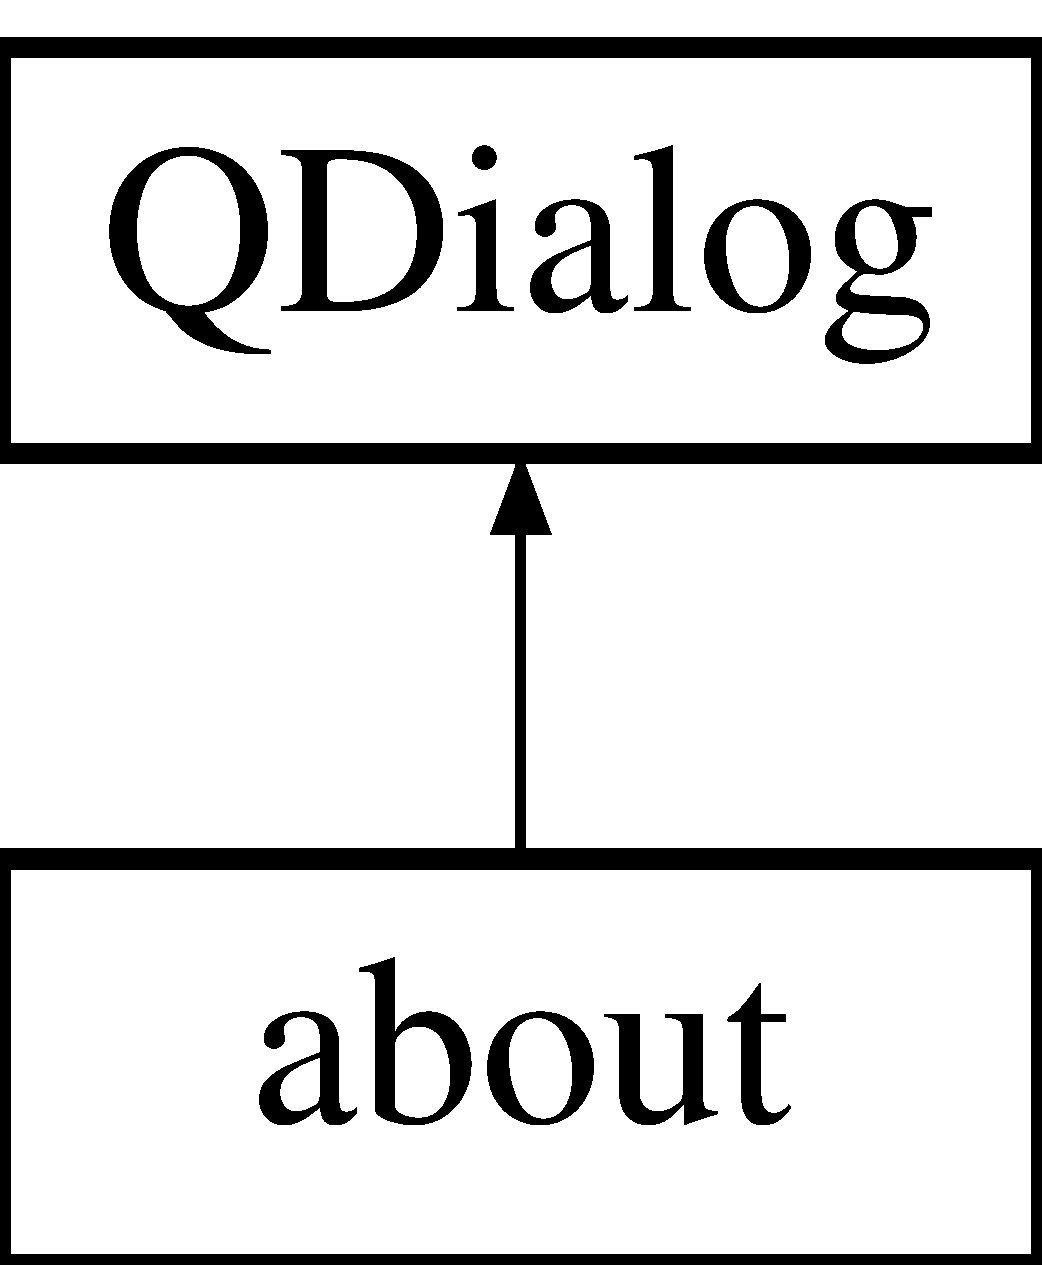
\includegraphics[height=2.000000cm]{classabout}
\end{center}
\end{figure}
\subsection*{Public Member Functions}
\begin{DoxyCompactItemize}
\item 
\hyperlink{classabout_ab16a8ec628d97aee17f0332e09964f52}{about} (Q\-Widget $\ast$parent=0)
\begin{DoxyCompactList}\small\item\em El contructor de la clase. \end{DoxyCompactList}\end{DoxyCompactItemize}


\subsection{Detailed Description}
The about es la clase que se encarga de mostrar la informacion en about del programa. 

\subsection{Constructor \& Destructor Documentation}
\hypertarget{classabout_ab16a8ec628d97aee17f0332e09964f52}{\index{about@{about}!about@{about}}
\index{about@{about}!about@{about}}
\subsubsection[{about}]{\setlength{\rightskip}{0pt plus 5cm}about\-::about (
\begin{DoxyParamCaption}
\item[{Q\-Widget $\ast$}]{parent = {\ttfamily 0}}
\end{DoxyParamCaption}
)\hspace{0.3cm}{\ttfamily [explicit]}}}\label{classabout_ab16a8ec628d97aee17f0332e09964f52}


El contructor de la clase. 


\begin{DoxyParams}{Parameters}
{\em } & \\
\hline
\end{DoxyParams}


The documentation for this class was generated from the following files\-:\begin{DoxyCompactItemize}
\item 
\hyperlink{about_8h}{about.\-h}\item 
about.\-cpp\end{DoxyCompactItemize}

\hypertarget{class_celda}{\section{Celda Class Reference}
\label{class_celda}\index{Celda@{Celda}}
}
Inheritance diagram for Celda\-:\begin{figure}[H]
\begin{center}
\leavevmode
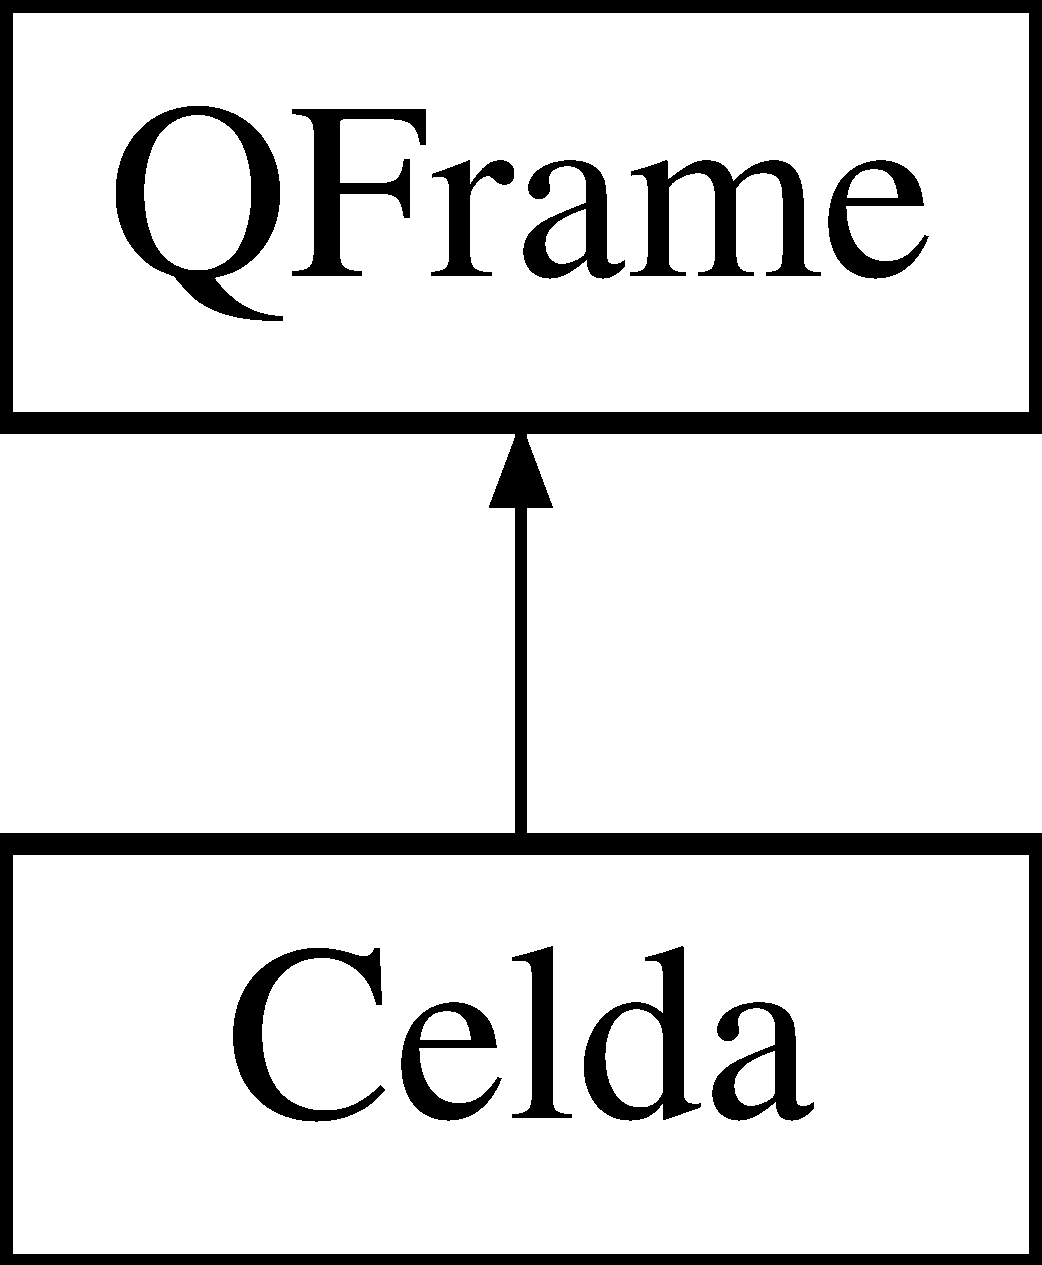
\includegraphics[height=2.000000cm]{class_celda}
\end{center}
\end{figure}
\subsection*{Signals}
\begin{DoxyCompactItemize}
\item 
\hypertarget{class_celda_a7f23df77ebd6ac50edb1e46101d2734a}{void {\bfseries clicked} ()}\label{class_celda_a7f23df77ebd6ac50edb1e46101d2734a}

\end{DoxyCompactItemize}
\subsection*{Public Member Functions}
\begin{DoxyCompactItemize}
\item 
\hyperlink{class_celda_a061c79d4a2ac8b4305d8bb989feec1cd}{Celda} (int value, Q\-Point poscicion)
\begin{DoxyCompactList}\small\item\em Crea una nueva celda en una posicion con un valor en ella. \end{DoxyCompactList}\item 
void \hyperlink{class_celda_a26dd4a943c3b516a00c3c3ec56bd56ac}{set\-Value} (int valor)
\begin{DoxyCompactList}\small\item\em cambia el valor de una celda \end{DoxyCompactList}\item 
void \hyperlink{class_celda_a11857539b9f49484bf5344fbe72288bb}{add\-Hint} (int valor)
\begin{DoxyCompactList}\small\item\em añade los hints al tablero \end{DoxyCompactList}\item 
void \hyperlink{class_celda_a2f36ec0296181ee26477fcdf049f2334}{set\-Lite} (int valor)
\begin{DoxyCompactList}\small\item\em set\-Lite \end{DoxyCompactList}\item 
\hypertarget{class_celda_a3e523de46ddbdb2d8497ad67c0009f1e}{void \hyperlink{class_celda_a3e523de46ddbdb2d8497ad67c0009f1e}{reset} ()}\label{class_celda_a3e523de46ddbdb2d8497ad67c0009f1e}

\begin{DoxyCompactList}\small\item\em reset \end{DoxyCompactList}\item 
\hypertarget{class_celda_ac93663c46fa34649bf44d3927c7f0ca1}{void {\bfseries check} ()}\label{class_celda_ac93663c46fa34649bf44d3927c7f0ca1}

\item 
\hypertarget{class_celda_a8420b9e44aed858bf90bc0ea8c0984fa}{void {\bfseries un\-Check} ()}\label{class_celda_a8420b9e44aed858bf90bc0ea8c0984fa}

\item 
\hypertarget{class_celda_af18a6e990908532034599a49784d4ff5}{void {\bfseries set\-Back\-Color} (Q\-String color)}\label{class_celda_af18a6e990908532034599a49784d4ff5}

\item 
\hypertarget{class_celda_ac56176d091cbca011a1d93530f179800}{void {\bfseries set\-Black\-Border} ()}\label{class_celda_ac56176d091cbca011a1d93530f179800}

\item 
\hypertarget{class_celda_aa37c81071e8d384b46661d30e30d9e3e}{int {\bfseries get\-Value} ()}\label{class_celda_aa37c81071e8d384b46661d30e30d9e3e}

\item 
\hypertarget{class_celda_a7e16d4f745601f63ac8e5178bc0f4e54}{int {\bfseries get\-Index} ()}\label{class_celda_a7e16d4f745601f63ac8e5178bc0f4e54}

\item 
\hypertarget{class_celda_a1018c36394dd882c632a71c7fb12999a}{int $\ast$ {\bfseries get\-Posibilities} ()}\label{class_celda_a1018c36394dd882c632a71c7fb12999a}

\item 
\hypertarget{class_celda_a592dd2bcba1d493d884c90b47fdadf00}{bool {\bfseries is\-Checked} ()}\label{class_celda_a592dd2bcba1d493d884c90b47fdadf00}

\item 
\hypertarget{class_celda_ab6966d037ddd5e0c1bb99aca39647379}{bool {\bfseries has\-Num} ()}\label{class_celda_ab6966d037ddd5e0c1bb99aca39647379}

\item 
\hypertarget{class_celda_a9de72cff68e6b39fb062b4a3d386f627}{Q\-Label $\ast$ {\bfseries get\-Number} ()}\label{class_celda_a9de72cff68e6b39fb062b4a3d386f627}

\end{DoxyCompactItemize}
\subsection*{Public Attributes}
\begin{DoxyCompactItemize}
\item 
\hypertarget{class_celda_ae7a0ff06a1409fc11aee254999108598}{Q\-Point {\bfseries pos}}\label{class_celda_ae7a0ff06a1409fc11aee254999108598}

\end{DoxyCompactItemize}
\subsection*{Protected Member Functions}
\begin{DoxyCompactItemize}
\item 
\hypertarget{class_celda_ae51d95d1ac700fcbb35e45ebea8be779}{void {\bfseries mouse\-Release\-Event} (Q\-Mouse\-Event $\ast$)}\label{class_celda_ae51d95d1ac700fcbb35e45ebea8be779}

\end{DoxyCompactItemize}


\subsection{Constructor \& Destructor Documentation}
\hypertarget{class_celda_a061c79d4a2ac8b4305d8bb989feec1cd}{\index{Celda@{Celda}!Celda@{Celda}}
\index{Celda@{Celda}!Celda@{Celda}}
\subsubsection[{Celda}]{\setlength{\rightskip}{0pt plus 5cm}Celda\-::\-Celda (
\begin{DoxyParamCaption}
\item[{int}]{value, }
\item[{Q\-Point}]{poscicion}
\end{DoxyParamCaption}
)\hspace{0.3cm}{\ttfamily [explicit]}}}\label{class_celda_a061c79d4a2ac8b4305d8bb989feec1cd}


Crea una nueva celda en una posicion con un valor en ella. 


\begin{DoxyParams}{Parameters}
{\em el} & valor de la casilla \\
\hline
{\em posicion} & en el tablero del sudoku \\
\hline
\end{DoxyParams}


\subsection{Member Function Documentation}
\hypertarget{class_celda_a11857539b9f49484bf5344fbe72288bb}{\index{Celda@{Celda}!add\-Hint@{add\-Hint}}
\index{add\-Hint@{add\-Hint}!Celda@{Celda}}
\subsubsection[{add\-Hint}]{\setlength{\rightskip}{0pt plus 5cm}void Celda\-::add\-Hint (
\begin{DoxyParamCaption}
\item[{int}]{valor}
\end{DoxyParamCaption}
)}}\label{class_celda_a11857539b9f49484bf5344fbe72288bb}


añade los hints al tablero 


\begin{DoxyParams}{Parameters}
{\em numero} & de hints que seran añadidos \\
\hline
\end{DoxyParams}
\hypertarget{class_celda_a2f36ec0296181ee26477fcdf049f2334}{\index{Celda@{Celda}!set\-Lite@{set\-Lite}}
\index{set\-Lite@{set\-Lite}!Celda@{Celda}}
\subsubsection[{set\-Lite}]{\setlength{\rightskip}{0pt plus 5cm}void Celda\-::set\-Lite (
\begin{DoxyParamCaption}
\item[{int}]{valor}
\end{DoxyParamCaption}
)}}\label{class_celda_a2f36ec0296181ee26477fcdf049f2334}


set\-Lite 


\begin{DoxyParams}{Parameters}
{\em valor} & \\
\hline
\end{DoxyParams}
\hypertarget{class_celda_a26dd4a943c3b516a00c3c3ec56bd56ac}{\index{Celda@{Celda}!set\-Value@{set\-Value}}
\index{set\-Value@{set\-Value}!Celda@{Celda}}
\subsubsection[{set\-Value}]{\setlength{\rightskip}{0pt plus 5cm}void Celda\-::set\-Value (
\begin{DoxyParamCaption}
\item[{int}]{valor}
\end{DoxyParamCaption}
)}}\label{class_celda_a26dd4a943c3b516a00c3c3ec56bd56ac}


cambia el valor de una celda 


\begin{DoxyParams}{Parameters}
{\em valor} & a colocar en la celda que se cambiara \\
\hline
\end{DoxyParams}


The documentation for this class was generated from the following files\-:\begin{DoxyCompactItemize}
\item 
\hyperlink{celda_8h}{celda.\-h}\item 
celda.\-cpp\end{DoxyCompactItemize}

\hypertarget{class_gen_matriz}{\section{Gen\-Matriz Class Reference}
\label{class_gen_matriz}\index{Gen\-Matriz@{Gen\-Matriz}}
}
\subsection*{Public Member Functions}
\begin{DoxyCompactItemize}
\item 
\hypertarget{class_gen_matriz_a8fac64f00cae60f47afbf6cf43346832}{\hyperlink{class_gen_matriz_a8fac64f00cae60f47afbf6cf43346832}{Gen\-Matriz} ()}\label{class_gen_matriz_a8fac64f00cae60f47afbf6cf43346832}

\begin{DoxyCompactList}\small\item\em El contructor de la clase \hyperlink{class_gen_matriz}{Gen\-Matriz}, crea un sudoku resuelto a partir de un algoritmo de semilla. \end{DoxyCompactList}\item 
\hypertarget{class_gen_matriz_ae4e6b5ed243424a06becc3b9296fe520}{void \hyperlink{class_gen_matriz_ae4e6b5ed243424a06becc3b9296fe520}{llenar\-Matriz\-Semilla} ()}\label{class_gen_matriz_ae4e6b5ed243424a06becc3b9296fe520}

\begin{DoxyCompactList}\small\item\em La funcion llenar\-Matriz\-Semilla es usada internamente en el constructor de la clase para setear un sudoku resuelto. \end{DoxyCompactList}\item 
\hypertarget{class_gen_matriz_a68e793d89185716f36367320262723eb}{void \hyperlink{class_gen_matriz_a68e793d89185716f36367320262723eb}{generar\-Matriz\-Sudoku} ()}\label{class_gen_matriz_a68e793d89185716f36367320262723eb}

\begin{DoxyCompactList}\small\item\em La funcion generar\-Matriz\-Sudoku se encarga de cambiar numeros, filasy columnas para generar sudokus diferentes. \end{DoxyCompactList}\item 
\hypertarget{class_gen_matriz_ac8b87d3d6f8402ce11b0e8c2e54267f4}{void \hyperlink{class_gen_matriz_ac8b87d3d6f8402ce11b0e8c2e54267f4}{generar\-Arreglos} ()}\label{class_gen_matriz_ac8b87d3d6f8402ce11b0e8c2e54267f4}

\begin{DoxyCompactList}\small\item\em La funcion generar\-Arreglos nos permite guardar la posicion de cada numero de la matriz. \end{DoxyCompactList}\item 
int \hyperlink{class_gen_matriz_af86ecf150e71673b7ed1e488f5f61efb}{arreglo\-De\-Numeros} (int i, int j)
\begin{DoxyCompactList}\small\item\em La funcion arreglo\-De\-Numeros retorna un valor de una matriz. \end{DoxyCompactList}\item 
void \hyperlink{class_gen_matriz_af5686320072f21d88b5fbc85963bc280}{guardar\-Pos\-Num} (int n, int fila, int columna)
\begin{DoxyCompactList}\small\item\em guardar\-Pos\-Num mantiene la poscicion de cada numero \end{DoxyCompactList}\item 
void \hyperlink{class_gen_matriz_ae58e92d9d0efc983f96b53a02f9cd8a5}{imprimir\-Matriz} (int matriz\mbox{[}9\mbox{]}\mbox{[}9\mbox{]})
\begin{DoxyCompactList}\small\item\em imprimir\-Matriz imprime una matriz de 9 x 9 \end{DoxyCompactList}\item 
void \hyperlink{class_gen_matriz_aa67088279c4f7a0877c6b128db8d0ff5}{colocar\-Numeros} (Q\-List$<$ int $>$ aleatorios)
\begin{DoxyCompactList}\small\item\em colocar\-Numeros ubica los valores en una nueva poscicion \end{DoxyCompactList}\end{DoxyCompactItemize}


\subsection{Member Function Documentation}
\hypertarget{class_gen_matriz_af86ecf150e71673b7ed1e488f5f61efb}{\index{Gen\-Matriz@{Gen\-Matriz}!arreglo\-De\-Numeros@{arreglo\-De\-Numeros}}
\index{arreglo\-De\-Numeros@{arreglo\-De\-Numeros}!GenMatriz@{Gen\-Matriz}}
\subsubsection[{arreglo\-De\-Numeros}]{\setlength{\rightskip}{0pt plus 5cm}int Gen\-Matriz\-::arreglo\-De\-Numeros (
\begin{DoxyParamCaption}
\item[{int}]{i, }
\item[{int}]{j}
\end{DoxyParamCaption}
)}}\label{class_gen_matriz_af86ecf150e71673b7ed1e488f5f61efb}


La funcion arreglo\-De\-Numeros retorna un valor de una matriz. 


\begin{DoxyParams}{Parameters}
{\em i} & es la posicion del subindice para la fila \\
\hline
{\em j} & es la posicion delsubindice para la columna \\
\hline
\end{DoxyParams}
\begin{DoxyReturn}{Returns}
retorna un entero con el valor de esa posicion en la matriz 
\end{DoxyReturn}
\hypertarget{class_gen_matriz_aa67088279c4f7a0877c6b128db8d0ff5}{\index{Gen\-Matriz@{Gen\-Matriz}!colocar\-Numeros@{colocar\-Numeros}}
\index{colocar\-Numeros@{colocar\-Numeros}!GenMatriz@{Gen\-Matriz}}
\subsubsection[{colocar\-Numeros}]{\setlength{\rightskip}{0pt plus 5cm}void Gen\-Matriz\-::colocar\-Numeros (
\begin{DoxyParamCaption}
\item[{Q\-List$<$ int $>$}]{aleatorios}
\end{DoxyParamCaption}
)}}\label{class_gen_matriz_aa67088279c4f7a0877c6b128db8d0ff5}


colocar\-Numeros ubica los valores en una nueva poscicion 


\begin{DoxyParams}{Parameters}
{\em aleatorios} & es la nueva poscicion de los numeros \\
\hline
\end{DoxyParams}
\hypertarget{class_gen_matriz_af5686320072f21d88b5fbc85963bc280}{\index{Gen\-Matriz@{Gen\-Matriz}!guardar\-Pos\-Num@{guardar\-Pos\-Num}}
\index{guardar\-Pos\-Num@{guardar\-Pos\-Num}!GenMatriz@{Gen\-Matriz}}
\subsubsection[{guardar\-Pos\-Num}]{\setlength{\rightskip}{0pt plus 5cm}void Gen\-Matriz\-::guardar\-Pos\-Num (
\begin{DoxyParamCaption}
\item[{int}]{n, }
\item[{int}]{fila, }
\item[{int}]{columna}
\end{DoxyParamCaption}
)}}\label{class_gen_matriz_af5686320072f21d88b5fbc85963bc280}


guardar\-Pos\-Num mantiene la poscicion de cada numero 


\begin{DoxyParams}{Parameters}
{\em n} & es el numero \\
\hline
{\em fila} & posicion de la fila en la matriz \\
\hline
{\em columna} & posicion de la columna de la matriz \\
\hline
\end{DoxyParams}
\hypertarget{class_gen_matriz_ae58e92d9d0efc983f96b53a02f9cd8a5}{\index{Gen\-Matriz@{Gen\-Matriz}!imprimir\-Matriz@{imprimir\-Matriz}}
\index{imprimir\-Matriz@{imprimir\-Matriz}!GenMatriz@{Gen\-Matriz}}
\subsubsection[{imprimir\-Matriz}]{\setlength{\rightskip}{0pt plus 5cm}void Gen\-Matriz\-::imprimir\-Matriz (
\begin{DoxyParamCaption}
\item[{int}]{matriz\mbox{[}9\mbox{]}\mbox{[}9\mbox{]}}
\end{DoxyParamCaption}
)}}\label{class_gen_matriz_ae58e92d9d0efc983f96b53a02f9cd8a5}


imprimir\-Matriz imprime una matriz de 9 x 9 


\begin{DoxyParams}{Parameters}
{\em matriz} & es la matriz a ser impresa \\
\hline
\end{DoxyParams}


The documentation for this class was generated from the following files\-:\begin{DoxyCompactItemize}
\item 
\hyperlink{genmatriz_8h}{genmatriz.\-h}\item 
genmatriz.\-cpp\end{DoxyCompactItemize}

\hypertarget{class_guardar}{\section{Guardar Class Reference}
\label{class_guardar}\index{Guardar@{Guardar}}
}


The \hyperlink{class_guardar}{Guardar} Es la clase encargada de guardar y cargar archivos.  




{\ttfamily \#include $<$guardar.\-h$>$}

\subsection*{Public Member Functions}
\begin{DoxyCompactItemize}
\item 
\hypertarget{class_guardar_a265efa37b91672b6040a27f2207192b7}{\hyperlink{class_guardar_a265efa37b91672b6040a27f2207192b7}{Guardar} ()}\label{class_guardar_a265efa37b91672b6040a27f2207192b7}

\begin{DoxyCompactList}\small\item\em \hyperlink{class_guardar}{Guardar} constructor de la clase guardar para guardar y leer archivos encriptados. \end{DoxyCompactList}\item 
\hypertarget{class_guardar_aa602d00edb44609652777954ad2f8c18}{void \hyperlink{class_guardar_aa602d00edb44609652777954ad2f8c18}{crear\-Archivo} ()}\label{class_guardar_aa602d00edb44609652777954ad2f8c18}

\begin{DoxyCompactList}\small\item\em crear\-Archivo abre la ventana default del sistema para explorar archivos y obtener la ruta \end{DoxyCompactList}\item 
void \hyperlink{class_guardar_ab2a0427431816fd0c1138afb7410856c}{guardar\-Valores} (int m\mbox{[}9\mbox{]}\mbox{[}9\mbox{]}, int sol\mbox{[}9\mbox{]}\mbox{[}9\mbox{]}, Q\-String jugador, Q\-String \hyperlink{classnivel}{nivel}, Q\-String tiempo)
\begin{DoxyCompactList}\small\item\em guardar\-Valores concatena todos los datos a ser guardados \end{DoxyCompactList}\item 
void \hyperlink{class_guardar_ad1893652f3dad094f002e8415b20b67e}{leer\-Archivo} (int m\mbox{[}9\mbox{]}\mbox{[}9\mbox{]}, int sol\mbox{[}9\mbox{]}\mbox{[}9\mbox{]}, Q\-String $\ast$name, Q\-String $\ast$level, Q\-Time $\ast$t)
\begin{DoxyCompactList}\small\item\em leer\-Archivo lee el archivo y usa una expresion regular para separar las distintas candenas \end{DoxyCompactList}\end{DoxyCompactItemize}


\subsection{Detailed Description}
The \hyperlink{class_guardar}{Guardar} Es la clase encargada de guardar y cargar archivos. 

\subsection{Member Function Documentation}
\hypertarget{class_guardar_ab2a0427431816fd0c1138afb7410856c}{\index{Guardar@{Guardar}!guardar\-Valores@{guardar\-Valores}}
\index{guardar\-Valores@{guardar\-Valores}!Guardar@{Guardar}}
\subsubsection[{guardar\-Valores}]{\setlength{\rightskip}{0pt plus 5cm}void Guardar\-::guardar\-Valores (
\begin{DoxyParamCaption}
\item[{int}]{m\mbox{[}9\mbox{]}\mbox{[}9\mbox{]}, }
\item[{int}]{sol\mbox{[}9\mbox{]}\mbox{[}9\mbox{]}, }
\item[{Q\-String}]{jugador, }
\item[{Q\-String}]{nivel, }
\item[{Q\-String}]{tiempo}
\end{DoxyParamCaption}
)}}\label{class_guardar_ab2a0427431816fd0c1138afb7410856c}


guardar\-Valores concatena todos los datos a ser guardados 


\begin{DoxyParams}{Parameters}
{\em m} & matriz que mantiene el avance del juego \\
\hline
{\em sol} & matriz con la solucion del juego \\
\hline
{\em jugador} & nombre del juagador \\
\hline
{\em nivel} & nivel en el que esta jugando \\
\hline
{\em tiempo} & tiempo acumulado del reloj \\
\hline
\end{DoxyParams}
\hypertarget{class_guardar_ad1893652f3dad094f002e8415b20b67e}{\index{Guardar@{Guardar}!leer\-Archivo@{leer\-Archivo}}
\index{leer\-Archivo@{leer\-Archivo}!Guardar@{Guardar}}
\subsubsection[{leer\-Archivo}]{\setlength{\rightskip}{0pt plus 5cm}void Guardar\-::leer\-Archivo (
\begin{DoxyParamCaption}
\item[{int}]{m\mbox{[}9\mbox{]}\mbox{[}9\mbox{]}, }
\item[{int}]{sol\mbox{[}9\mbox{]}\mbox{[}9\mbox{]}, }
\item[{Q\-String $\ast$}]{name, }
\item[{Q\-String $\ast$}]{level, }
\item[{Q\-Time $\ast$}]{t}
\end{DoxyParamCaption}
)}}\label{class_guardar_ad1893652f3dad094f002e8415b20b67e}


leer\-Archivo lee el archivo y usa una expresion regular para separar las distintas candenas 


\begin{DoxyParams}{Parameters}
{\em m} & setea en esta el avance del juego \\
\hline
{\em sol} & setea en sol la solucion del juego \\
\hline
{\em name} & para setear el nombre del jugador \\
\hline
{\em level} & para setear el nivel del jugador \\
\hline
{\em t} & para setear el tiempo del juegador \\
\hline
\end{DoxyParams}


The documentation for this class was generated from the following files\-:\begin{DoxyCompactItemize}
\item 
\hyperlink{guardar_8h}{guardar.\-h}\item 
guardar.\-cpp\end{DoxyCompactItemize}

\hypertarget{class_main_table}{\section{Main\-Table Class Reference}
\label{class_main_table}\index{Main\-Table@{Main\-Table}}
}
Inheritance diagram for Main\-Table\-:\begin{figure}[H]
\begin{center}
\leavevmode
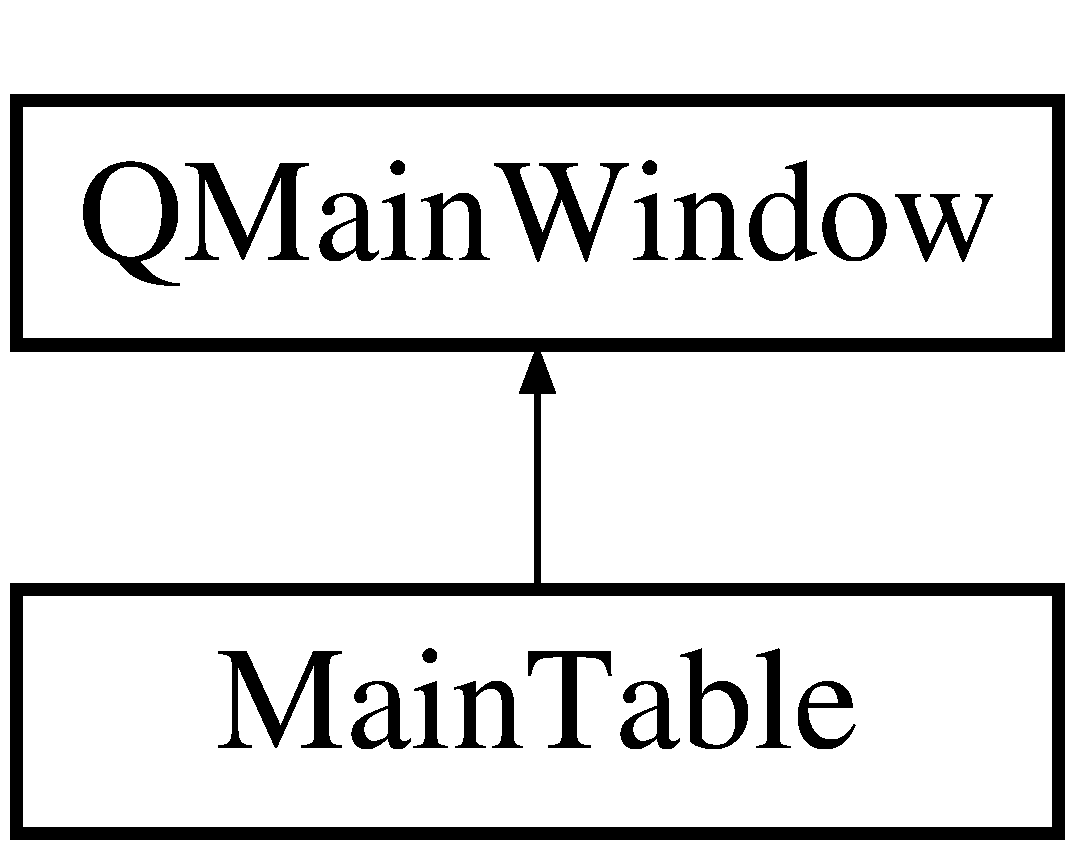
\includegraphics[height=2.000000cm]{class_main_table}
\end{center}
\end{figure}
\subsection*{Public Member Functions}
\begin{DoxyCompactItemize}
\item 
\hypertarget{class_main_table_a536fdc279aa0ed4e14cc25ab6f89a74d}{{\bfseries Main\-Table} (Q\-Widget $\ast$parent=0)}\label{class_main_table_a536fdc279aa0ed4e14cc25ab6f89a74d}

\end{DoxyCompactItemize}


The documentation for this class was generated from the following files\-:\begin{DoxyCompactItemize}
\item 
\hyperlink{maintable_8h}{maintable.\-h}\item 
maintable.\-cpp\end{DoxyCompactItemize}

\hypertarget{classnivel}{\section{nivel Class Reference}
\label{classnivel}\index{nivel@{nivel}}
}


The nivel esta clase s para emitir diferentes señales segun el nivel de dificultad que el usuario elija.  




{\ttfamily \#include $<$nivel.\-h$>$}

Inheritance diagram for nivel\-:\begin{figure}[H]
\begin{center}
\leavevmode
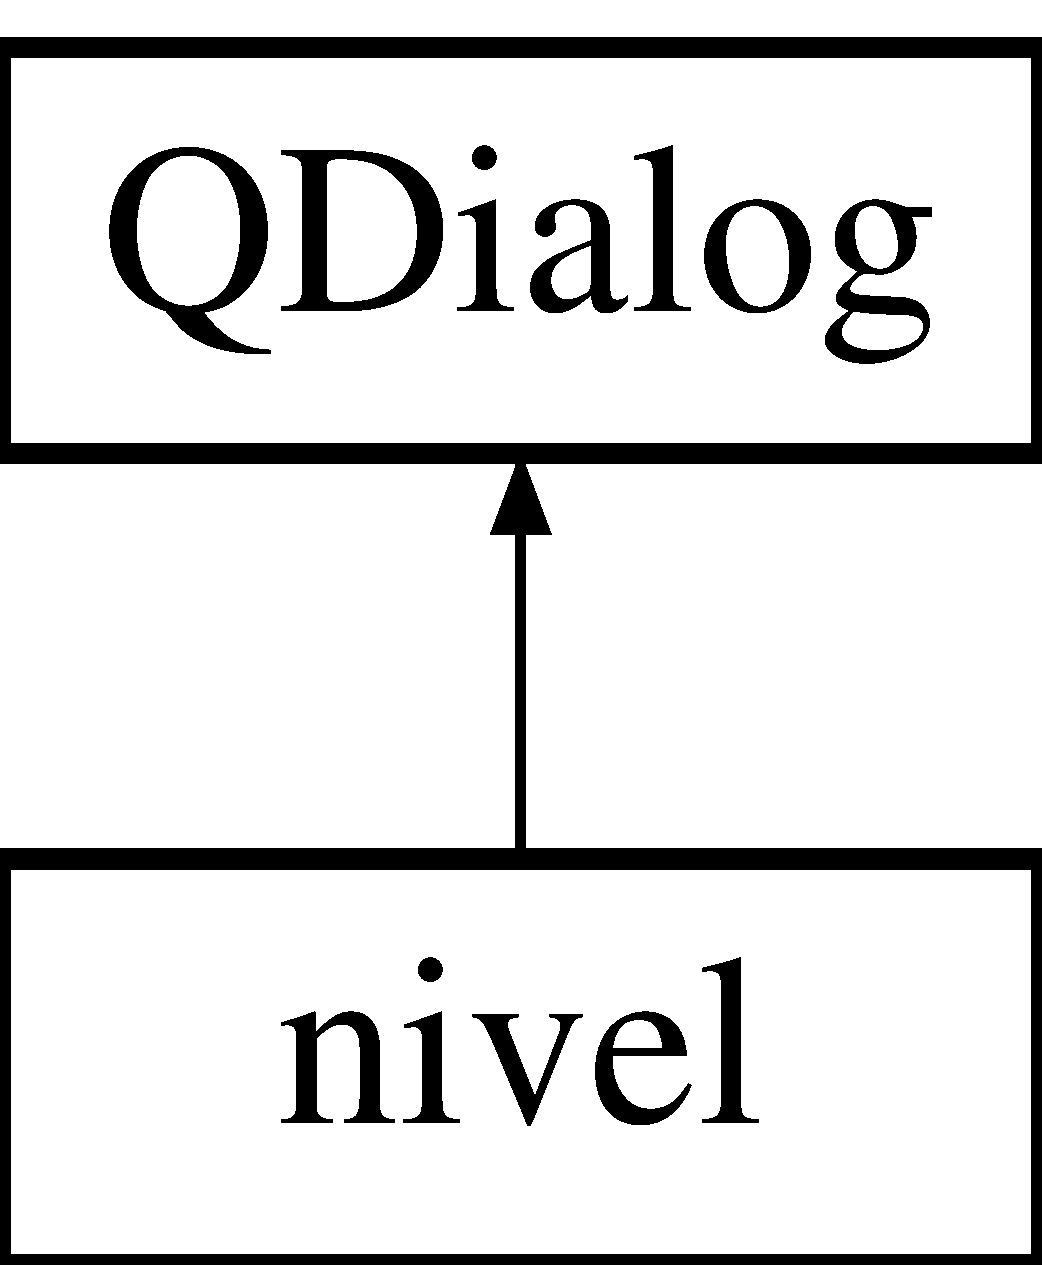
\includegraphics[height=2.000000cm]{classnivel}
\end{center}
\end{figure}
\subsection*{Signals}
\begin{DoxyCompactItemize}
\item 
void \hyperlink{classnivel_a8a46a97c07c0cc03939e26108e9ffb80}{app\-Ready} (int i)
\begin{DoxyCompactList}\small\item\em app\-Ready registra el slot que emitio la señal \end{DoxyCompactList}\end{DoxyCompactItemize}
\subsection*{Public Member Functions}
\begin{DoxyCompactItemize}
\item 
\hypertarget{classnivel_add84530f153521109b3c306edf61db1d}{{\bfseries nivel} (Q\-Widget $\ast$parent=0)}\label{classnivel_add84530f153521109b3c306edf61db1d}

\end{DoxyCompactItemize}


\subsection{Detailed Description}
The nivel esta clase s para emitir diferentes señales segun el nivel de dificultad que el usuario elija. 

\subsection{Member Function Documentation}
\hypertarget{classnivel_a8a46a97c07c0cc03939e26108e9ffb80}{\index{nivel@{nivel}!app\-Ready@{app\-Ready}}
\index{app\-Ready@{app\-Ready}!nivel@{nivel}}
\subsubsection[{app\-Ready}]{\setlength{\rightskip}{0pt plus 5cm}void nivel\-::app\-Ready (
\begin{DoxyParamCaption}
\item[{int}]{i}
\end{DoxyParamCaption}
)\hspace{0.3cm}{\ttfamily [signal]}}}\label{classnivel_a8a46a97c07c0cc03939e26108e9ffb80}


app\-Ready registra el slot que emitio la señal 


\begin{DoxyParams}{Parameters}
{\em parametro} & de entrada de la señal \\
\hline
\end{DoxyParams}


The documentation for this class was generated from the following files\-:\begin{DoxyCompactItemize}
\item 
\hyperlink{nivel_8h}{nivel.\-h}\item 
nivel.\-cpp\end{DoxyCompactItemize}

\hypertarget{class_simple_crypt}{\section{Simple\-Crypt Class Reference}
\label{class_simple_crypt}\index{Simple\-Crypt@{Simple\-Crypt}}
}


Simple encryption and decryption of strings and byte arrays.  




{\ttfamily \#include $<$simplecrypt.\-h$>$}

\subsection*{Public Types}
\begin{DoxyCompactItemize}
\item 
enum \hyperlink{class_simple_crypt_a25298e746f175cf175a18f082092ca8e}{Compression\-Mode} \{ \hyperlink{class_simple_crypt_a25298e746f175cf175a18f082092ca8ea8d04b76ed73553456ec87e88b18ddc66}{Compression\-Auto}, 
\hyperlink{class_simple_crypt_a25298e746f175cf175a18f082092ca8ea10aec29129f4e6d08c4f61d7008ec8f7}{Compression\-Always}, 
\hyperlink{class_simple_crypt_a25298e746f175cf175a18f082092ca8eadc794d925e3af54dcef9a24ee3f60f6d}{Compression\-Never}
 \}
\item 
enum \hyperlink{class_simple_crypt_a42a5172e558d346b28421cc4e85feb2d}{Integrity\-Protection\-Mode} \{ \hyperlink{class_simple_crypt_a42a5172e558d346b28421cc4e85feb2da75547c41ccde1fb3d4db9f8c27164e4c}{Protection\-None}, 
\hyperlink{class_simple_crypt_a42a5172e558d346b28421cc4e85feb2dab6ccee9e9680f70c79213647c7814e5c}{Protection\-Checksum}, 
\hyperlink{class_simple_crypt_a42a5172e558d346b28421cc4e85feb2daf915c42837795744edbc5254eb93154f}{Protection\-Hash}
 \}
\item 
enum \hyperlink{class_simple_crypt_ab7f81049e78f021b55a36f7cfac5a09b}{Error} \{ \hyperlink{class_simple_crypt_ab7f81049e78f021b55a36f7cfac5a09ba77b7389ae8659e97df448c8fff79ca83}{Error\-No\-Error}, 
\hyperlink{class_simple_crypt_ab7f81049e78f021b55a36f7cfac5a09bacfb6271ef5415fe5e6a0e5ee3094f3a7}{Error\-No\-Key\-Set}, 
\hyperlink{class_simple_crypt_ab7f81049e78f021b55a36f7cfac5a09ba4c43644f04a0eefc3ed2205223f19479}{Error\-Unknown\-Version}, 
\hyperlink{class_simple_crypt_ab7f81049e78f021b55a36f7cfac5a09ba8566157b59e4662d0400b34249918e88}{Error\-Integrity\-Failed}
 \}
\item 
enum {\bfseries Crypto\-Flag} \{ {\bfseries Crypto\-Flag\-None} = 0, 
{\bfseries Crypto\-Flag\-Compression} = 0x01, 
{\bfseries Crypto\-Flag\-Checksum} = 0x02, 
{\bfseries Crypto\-Flag\-Hash} = 0x04
 \}
\end{DoxyCompactItemize}
\subsection*{Public Member Functions}
\begin{DoxyCompactItemize}
\item 
\hyperlink{class_simple_crypt_ac474d12cfa9f93bfecea35891831046d}{Simple\-Crypt} ()
\item 
\hyperlink{class_simple_crypt_a65942757b85b3dd36618ea3edc5ceb89}{Simple\-Crypt} (quint64 key)
\item 
void \hyperlink{class_simple_crypt_aa7aad9ed2e88b883ba9214c7d9928745}{set\-Key} (quint64 key)
\item 
bool \hyperlink{class_simple_crypt_aa7cab41b041f1fbe1c62e484fea895ce}{has\-Key} () const 
\item 
void \hyperlink{class_simple_crypt_adc6c6355aa276c0d3516f7ad273f063b}{set\-Compression\-Mode} (\hyperlink{class_simple_crypt_a25298e746f175cf175a18f082092ca8e}{Compression\-Mode} mode)
\item 
\hyperlink{class_simple_crypt_a25298e746f175cf175a18f082092ca8e}{Compression\-Mode} \hyperlink{class_simple_crypt_a303253756b925678e53bafc8b72a4e96}{compression\-Mode} () const 
\item 
void \hyperlink{class_simple_crypt_a4fef5e6d3246ee57d6a7b68475b12b8b}{set\-Integrity\-Protection\-Mode} (\hyperlink{class_simple_crypt_a42a5172e558d346b28421cc4e85feb2d}{Integrity\-Protection\-Mode} mode)
\item 
\hyperlink{class_simple_crypt_a42a5172e558d346b28421cc4e85feb2d}{Integrity\-Protection\-Mode} \hyperlink{class_simple_crypt_a81929610d0fd5667db83603f396ddb66}{integrity\-Protection\-Mode} () const 
\item 
\hyperlink{class_simple_crypt_ab7f81049e78f021b55a36f7cfac5a09b}{Error} \hyperlink{class_simple_crypt_a123562e29377ab26e3b398b588f596d9}{last\-Error} () const 
\item 
Q\-String \hyperlink{class_simple_crypt_af26a3d3c6cef9732190c1d2c6a53a5b5}{encrypt\-To\-String} (const Q\-String \&plaintext)
\item 
Q\-String \hyperlink{class_simple_crypt_aa72b79bf7a5bb971bf3b0a52b9247efd}{encrypt\-To\-String} (Q\-Byte\-Array plaintext)
\item 
Q\-Byte\-Array \hyperlink{class_simple_crypt_ae1991c7748b2bb74468bee0be372d2c4}{encrypt\-To\-Byte\-Array} (const Q\-String \&plaintext)
\item 
Q\-Byte\-Array \hyperlink{class_simple_crypt_a741305d04e86bcb7d4625b05bf234887}{encrypt\-To\-Byte\-Array} (Q\-Byte\-Array plaintext)
\item 
Q\-String \hyperlink{class_simple_crypt_aa454cf372b534fd5ffaa2c5bd0fa57ea}{decrypt\-To\-String} (const Q\-String \&cyphertext)
\item 
Q\-Byte\-Array \hyperlink{class_simple_crypt_ad6785e087d449a1aa80c39248e98fcda}{decrypt\-To\-Byte\-Array} (const Q\-String \&cyphertext)
\item 
Q\-String \hyperlink{class_simple_crypt_ad1a3257cefee43773803ec1b12654f92}{decrypt\-To\-String} (Q\-Byte\-Array cypher)
\item 
Q\-Byte\-Array \hyperlink{class_simple_crypt_a4babb69e45849f672574a26b6433c85a}{decrypt\-To\-Byte\-Array} (Q\-Byte\-Array cypher)
\item 
\hypertarget{class_simple_crypt_a710fb3871372ccddd6450f73afca24eb}{{\bfseries Q\-\_\-\-D\-E\-C\-L\-A\-R\-E\-\_\-\-F\-L\-A\-G\-S} (Crypto\-Flags, Crypto\-Flag)}\label{class_simple_crypt_a710fb3871372ccddd6450f73afca24eb}

\end{DoxyCompactItemize}


\subsection{Detailed Description}
Simple encryption and decryption of strings and byte arrays. 

This class provides a simple implementation of encryption and decryption of strings and byte arrays.

\begin{DoxyWarning}{Warning}
The encryption provided by this class is N\-O\-T strong encryption. It may help to shield things from curious eyes, but it will N\-O\-T stand up to someone determined to break the encryption. Don't say you were not warned.
\end{DoxyWarning}
The class uses a 64 bit key. Simply create an instance of the class, set the key, and use the \hyperlink{class_simple_crypt_af26a3d3c6cef9732190c1d2c6a53a5b5}{encrypt\-To\-String()} method to calculate an encrypted version of the input string. To decrypt that string again, use an instance of \hyperlink{class_simple_crypt}{Simple\-Crypt} initialized with the same key, and call the \hyperlink{class_simple_crypt_aa454cf372b534fd5ffaa2c5bd0fa57ea}{decrypt\-To\-String()} method with the encrypted string. If the key matches, the decrypted version of the string will be returned again.

If you do not provide a key, or if something else is wrong, the encryption and decryption function will return an empty string or will return a string containing nonsense. \hyperlink{class_simple_crypt_a123562e29377ab26e3b398b588f596d9}{last\-Error()} will return a value indicating if the method was succesful, and if not, why not.

\hyperlink{class_simple_crypt}{Simple\-Crypt} is prepared for the case that the encryption and decryption algorithm is changed in a later version, by prepending a version identifier to the cypertext. 

\subsection{Member Enumeration Documentation}
\hypertarget{class_simple_crypt_a25298e746f175cf175a18f082092ca8e}{\index{Simple\-Crypt@{Simple\-Crypt}!Compression\-Mode@{Compression\-Mode}}
\index{Compression\-Mode@{Compression\-Mode}!SimpleCrypt@{Simple\-Crypt}}
\subsubsection[{Compression\-Mode}]{\setlength{\rightskip}{0pt plus 5cm}enum {\bf Simple\-Crypt\-::\-Compression\-Mode}}}\label{class_simple_crypt_a25298e746f175cf175a18f082092ca8e}
Compression\-Mode describes if compression will be applied to the data to be encrypted. \begin{Desc}
\item[Enumerator]\par
\begin{description}
\index{Compression\-Auto@{Compression\-Auto}!Simple\-Crypt@{Simple\-Crypt}}\index{Simple\-Crypt@{Simple\-Crypt}!Compression\-Auto@{Compression\-Auto}}\item[{\em 
\hypertarget{class_simple_crypt_a25298e746f175cf175a18f082092ca8ea8d04b76ed73553456ec87e88b18ddc66}{Compression\-Auto}\label{class_simple_crypt_a25298e746f175cf175a18f082092ca8ea8d04b76ed73553456ec87e88b18ddc66}
}]Only apply compression if that results in a shorter plaintext. \index{Compression\-Always@{Compression\-Always}!Simple\-Crypt@{Simple\-Crypt}}\index{Simple\-Crypt@{Simple\-Crypt}!Compression\-Always@{Compression\-Always}}\item[{\em 
\hypertarget{class_simple_crypt_a25298e746f175cf175a18f082092ca8ea10aec29129f4e6d08c4f61d7008ec8f7}{Compression\-Always}\label{class_simple_crypt_a25298e746f175cf175a18f082092ca8ea10aec29129f4e6d08c4f61d7008ec8f7}
}]Always apply compression. Note that for short inputs, a compression may result in longer data \index{Compression\-Never@{Compression\-Never}!Simple\-Crypt@{Simple\-Crypt}}\index{Simple\-Crypt@{Simple\-Crypt}!Compression\-Never@{Compression\-Never}}\item[{\em 
\hypertarget{class_simple_crypt_a25298e746f175cf175a18f082092ca8eadc794d925e3af54dcef9a24ee3f60f6d}{Compression\-Never}\label{class_simple_crypt_a25298e746f175cf175a18f082092ca8eadc794d925e3af54dcef9a24ee3f60f6d}
}]Never apply compression. \end{description}
\end{Desc}
\hypertarget{class_simple_crypt_ab7f81049e78f021b55a36f7cfac5a09b}{\index{Simple\-Crypt@{Simple\-Crypt}!Error@{Error}}
\index{Error@{Error}!SimpleCrypt@{Simple\-Crypt}}
\subsubsection[{Error}]{\setlength{\rightskip}{0pt plus 5cm}enum {\bf Simple\-Crypt\-::\-Error}}}\label{class_simple_crypt_ab7f81049e78f021b55a36f7cfac5a09b}
Error describes the type of error that occured. \begin{Desc}
\item[Enumerator]\par
\begin{description}
\index{Error\-No\-Error@{Error\-No\-Error}!Simple\-Crypt@{Simple\-Crypt}}\index{Simple\-Crypt@{Simple\-Crypt}!Error\-No\-Error@{Error\-No\-Error}}\item[{\em 
\hypertarget{class_simple_crypt_ab7f81049e78f021b55a36f7cfac5a09ba77b7389ae8659e97df448c8fff79ca83}{Error\-No\-Error}\label{class_simple_crypt_ab7f81049e78f021b55a36f7cfac5a09ba77b7389ae8659e97df448c8fff79ca83}
}]No error occurred. \index{Error\-No\-Key\-Set@{Error\-No\-Key\-Set}!Simple\-Crypt@{Simple\-Crypt}}\index{Simple\-Crypt@{Simple\-Crypt}!Error\-No\-Key\-Set@{Error\-No\-Key\-Set}}\item[{\em 
\hypertarget{class_simple_crypt_ab7f81049e78f021b55a36f7cfac5a09bacfb6271ef5415fe5e6a0e5ee3094f3a7}{Error\-No\-Key\-Set}\label{class_simple_crypt_ab7f81049e78f021b55a36f7cfac5a09bacfb6271ef5415fe5e6a0e5ee3094f3a7}
}]No key was set. You can not encrypt or decrypt without a valid key. \index{Error\-Unknown\-Version@{Error\-Unknown\-Version}!Simple\-Crypt@{Simple\-Crypt}}\index{Simple\-Crypt@{Simple\-Crypt}!Error\-Unknown\-Version@{Error\-Unknown\-Version}}\item[{\em 
\hypertarget{class_simple_crypt_ab7f81049e78f021b55a36f7cfac5a09ba4c43644f04a0eefc3ed2205223f19479}{Error\-Unknown\-Version}\label{class_simple_crypt_ab7f81049e78f021b55a36f7cfac5a09ba4c43644f04a0eefc3ed2205223f19479}
}]The version of this data is unknown, or the data is otherwise not valid. \index{Error\-Integrity\-Failed@{Error\-Integrity\-Failed}!Simple\-Crypt@{Simple\-Crypt}}\index{Simple\-Crypt@{Simple\-Crypt}!Error\-Integrity\-Failed@{Error\-Integrity\-Failed}}\item[{\em 
\hypertarget{class_simple_crypt_ab7f81049e78f021b55a36f7cfac5a09ba8566157b59e4662d0400b34249918e88}{Error\-Integrity\-Failed}\label{class_simple_crypt_ab7f81049e78f021b55a36f7cfac5a09ba8566157b59e4662d0400b34249918e88}
}]The integrity check of the data failed. Perhaps the wrong key was used. \end{description}
\end{Desc}
\hypertarget{class_simple_crypt_a42a5172e558d346b28421cc4e85feb2d}{\index{Simple\-Crypt@{Simple\-Crypt}!Integrity\-Protection\-Mode@{Integrity\-Protection\-Mode}}
\index{Integrity\-Protection\-Mode@{Integrity\-Protection\-Mode}!SimpleCrypt@{Simple\-Crypt}}
\subsubsection[{Integrity\-Protection\-Mode}]{\setlength{\rightskip}{0pt plus 5cm}enum {\bf Simple\-Crypt\-::\-Integrity\-Protection\-Mode}}}\label{class_simple_crypt_a42a5172e558d346b28421cc4e85feb2d}
Integrity\-Protection\-Mode describes measures taken to make it possible to detect problems with the data or wrong decryption keys.

Measures involve adding a checksum or a cryptograhpic hash to the data to be encrypted. This increases the length of the resulting cypertext, but makes it possible to check if the plaintext appears to be valid after decryption. \begin{Desc}
\item[Enumerator]\par
\begin{description}
\index{Protection\-None@{Protection\-None}!Simple\-Crypt@{Simple\-Crypt}}\index{Simple\-Crypt@{Simple\-Crypt}!Protection\-None@{Protection\-None}}\item[{\em 
\hypertarget{class_simple_crypt_a42a5172e558d346b28421cc4e85feb2da75547c41ccde1fb3d4db9f8c27164e4c}{Protection\-None}\label{class_simple_crypt_a42a5172e558d346b28421cc4e85feb2da75547c41ccde1fb3d4db9f8c27164e4c}
}]The integerity of the encrypted data is not protected. It is not really possible to detect a wrong key, for instance. \index{Protection\-Checksum@{Protection\-Checksum}!Simple\-Crypt@{Simple\-Crypt}}\index{Simple\-Crypt@{Simple\-Crypt}!Protection\-Checksum@{Protection\-Checksum}}\item[{\em 
\hypertarget{class_simple_crypt_a42a5172e558d346b28421cc4e85feb2dab6ccee9e9680f70c79213647c7814e5c}{Protection\-Checksum}\label{class_simple_crypt_a42a5172e558d346b28421cc4e85feb2dab6ccee9e9680f70c79213647c7814e5c}
}]A simple checksum is used to verify that the data is in order. If not, an empty string is returned. \index{Protection\-Hash@{Protection\-Hash}!Simple\-Crypt@{Simple\-Crypt}}\index{Simple\-Crypt@{Simple\-Crypt}!Protection\-Hash@{Protection\-Hash}}\item[{\em 
\hypertarget{class_simple_crypt_a42a5172e558d346b28421cc4e85feb2daf915c42837795744edbc5254eb93154f}{Protection\-Hash}\label{class_simple_crypt_a42a5172e558d346b28421cc4e85feb2daf915c42837795744edbc5254eb93154f}
}]A cryptographic hash is used to verify the integrity of the data. This method produces a much stronger, but longer check \end{description}
\end{Desc}


\subsection{Constructor \& Destructor Documentation}
\hypertarget{class_simple_crypt_ac474d12cfa9f93bfecea35891831046d}{\index{Simple\-Crypt@{Simple\-Crypt}!Simple\-Crypt@{Simple\-Crypt}}
\index{Simple\-Crypt@{Simple\-Crypt}!SimpleCrypt@{Simple\-Crypt}}
\subsubsection[{Simple\-Crypt}]{\setlength{\rightskip}{0pt plus 5cm}Simple\-Crypt\-::\-Simple\-Crypt (
\begin{DoxyParamCaption}
{}
\end{DoxyParamCaption}
)}}\label{class_simple_crypt_ac474d12cfa9f93bfecea35891831046d}
Constructor.

Constructs a \hyperlink{class_simple_crypt}{Simple\-Crypt} instance without a valid key set on it. \hypertarget{class_simple_crypt_a65942757b85b3dd36618ea3edc5ceb89}{\index{Simple\-Crypt@{Simple\-Crypt}!Simple\-Crypt@{Simple\-Crypt}}
\index{Simple\-Crypt@{Simple\-Crypt}!SimpleCrypt@{Simple\-Crypt}}
\subsubsection[{Simple\-Crypt}]{\setlength{\rightskip}{0pt plus 5cm}Simple\-Crypt\-::\-Simple\-Crypt (
\begin{DoxyParamCaption}
\item[{quint64}]{key}
\end{DoxyParamCaption}
)\hspace{0.3cm}{\ttfamily [explicit]}}}\label{class_simple_crypt_a65942757b85b3dd36618ea3edc5ceb89}
Constructor.

Constructs a \hyperlink{class_simple_crypt}{Simple\-Crypt} instance and initializes it with the given\begin{DoxyItemize}
\item key. \end{DoxyItemize}


\subsection{Member Function Documentation}
\hypertarget{class_simple_crypt_a303253756b925678e53bafc8b72a4e96}{\index{Simple\-Crypt@{Simple\-Crypt}!compression\-Mode@{compression\-Mode}}
\index{compression\-Mode@{compression\-Mode}!SimpleCrypt@{Simple\-Crypt}}
\subsubsection[{compression\-Mode}]{\setlength{\rightskip}{0pt plus 5cm}{\bf Compression\-Mode} Simple\-Crypt\-::compression\-Mode (
\begin{DoxyParamCaption}
{}
\end{DoxyParamCaption}
) const\hspace{0.3cm}{\ttfamily [inline]}}}\label{class_simple_crypt_a303253756b925678e53bafc8b72a4e96}
Returns the Compression\-Mode that is currently in use. \hypertarget{class_simple_crypt_ad6785e087d449a1aa80c39248e98fcda}{\index{Simple\-Crypt@{Simple\-Crypt}!decrypt\-To\-Byte\-Array@{decrypt\-To\-Byte\-Array}}
\index{decrypt\-To\-Byte\-Array@{decrypt\-To\-Byte\-Array}!SimpleCrypt@{Simple\-Crypt}}
\subsubsection[{decrypt\-To\-Byte\-Array}]{\setlength{\rightskip}{0pt plus 5cm}Q\-Byte\-Array Simple\-Crypt\-::decrypt\-To\-Byte\-Array (
\begin{DoxyParamCaption}
\item[{const Q\-String \&}]{cyphertext}
\end{DoxyParamCaption}
)}}\label{class_simple_crypt_ad6785e087d449a1aa80c39248e98fcda}
Decrypts a cyphertext string encrypted with this class with the set key back to the plain text version.

If an error occured, such as non-\/matching keys between encryption and decryption, an empty string or a string containing nonsense may be returned. \hypertarget{class_simple_crypt_a4babb69e45849f672574a26b6433c85a}{\index{Simple\-Crypt@{Simple\-Crypt}!decrypt\-To\-Byte\-Array@{decrypt\-To\-Byte\-Array}}
\index{decrypt\-To\-Byte\-Array@{decrypt\-To\-Byte\-Array}!SimpleCrypt@{Simple\-Crypt}}
\subsubsection[{decrypt\-To\-Byte\-Array}]{\setlength{\rightskip}{0pt plus 5cm}Q\-Byte\-Array Simple\-Crypt\-::decrypt\-To\-Byte\-Array (
\begin{DoxyParamCaption}
\item[{Q\-Byte\-Array}]{cypher}
\end{DoxyParamCaption}
)}}\label{class_simple_crypt_a4babb69e45849f672574a26b6433c85a}
Decrypts a cyphertext binary encrypted with this class with the set key back to the plain text version.

If an error occured, such as non-\/matching keys between encryption and decryption, an empty string or a string containing nonsense may be returned. \hypertarget{class_simple_crypt_aa454cf372b534fd5ffaa2c5bd0fa57ea}{\index{Simple\-Crypt@{Simple\-Crypt}!decrypt\-To\-String@{decrypt\-To\-String}}
\index{decrypt\-To\-String@{decrypt\-To\-String}!SimpleCrypt@{Simple\-Crypt}}
\subsubsection[{decrypt\-To\-String}]{\setlength{\rightskip}{0pt plus 5cm}Q\-String Simple\-Crypt\-::decrypt\-To\-String (
\begin{DoxyParamCaption}
\item[{const Q\-String \&}]{cyphertext}
\end{DoxyParamCaption}
)}}\label{class_simple_crypt_aa454cf372b534fd5ffaa2c5bd0fa57ea}
Decrypts a cyphertext string encrypted with this class with the set key back to the plain text version.

If an error occured, such as non-\/matching keys between encryption and decryption, an empty string or a string containing nonsense may be returned. \hypertarget{class_simple_crypt_ad1a3257cefee43773803ec1b12654f92}{\index{Simple\-Crypt@{Simple\-Crypt}!decrypt\-To\-String@{decrypt\-To\-String}}
\index{decrypt\-To\-String@{decrypt\-To\-String}!SimpleCrypt@{Simple\-Crypt}}
\subsubsection[{decrypt\-To\-String}]{\setlength{\rightskip}{0pt plus 5cm}Q\-String Simple\-Crypt\-::decrypt\-To\-String (
\begin{DoxyParamCaption}
\item[{Q\-Byte\-Array}]{cypher}
\end{DoxyParamCaption}
)}}\label{class_simple_crypt_ad1a3257cefee43773803ec1b12654f92}
Decrypts a cyphertext binary encrypted with this class with the set key back to the plain text version.

If an error occured, such as non-\/matching keys between encryption and decryption, an empty string or a string containing nonsense may be returned. \hypertarget{class_simple_crypt_ae1991c7748b2bb74468bee0be372d2c4}{\index{Simple\-Crypt@{Simple\-Crypt}!encrypt\-To\-Byte\-Array@{encrypt\-To\-Byte\-Array}}
\index{encrypt\-To\-Byte\-Array@{encrypt\-To\-Byte\-Array}!SimpleCrypt@{Simple\-Crypt}}
\subsubsection[{encrypt\-To\-Byte\-Array}]{\setlength{\rightskip}{0pt plus 5cm}Q\-Byte\-Array Simple\-Crypt\-::encrypt\-To\-Byte\-Array (
\begin{DoxyParamCaption}
\item[{const Q\-String \&}]{plaintext}
\end{DoxyParamCaption}
)}}\label{class_simple_crypt_ae1991c7748b2bb74468bee0be372d2c4}
Encrypts the\begin{DoxyItemize}
\item plaintext string with the key the class was initialized with, and returns a binary cyphertext in a Q\-Byte\-Array the result.\end{DoxyItemize}
This method returns a byte array, that is useable for storing a binary format. If you need a string you can store in a text file, use \hyperlink{class_simple_crypt_af26a3d3c6cef9732190c1d2c6a53a5b5}{encrypt\-To\-String()} instead. \hypertarget{class_simple_crypt_a741305d04e86bcb7d4625b05bf234887}{\index{Simple\-Crypt@{Simple\-Crypt}!encrypt\-To\-Byte\-Array@{encrypt\-To\-Byte\-Array}}
\index{encrypt\-To\-Byte\-Array@{encrypt\-To\-Byte\-Array}!SimpleCrypt@{Simple\-Crypt}}
\subsubsection[{encrypt\-To\-Byte\-Array}]{\setlength{\rightskip}{0pt plus 5cm}Q\-Byte\-Array Simple\-Crypt\-::encrypt\-To\-Byte\-Array (
\begin{DoxyParamCaption}
\item[{Q\-Byte\-Array}]{plaintext}
\end{DoxyParamCaption}
)}}\label{class_simple_crypt_a741305d04e86bcb7d4625b05bf234887}
Encrypts the\begin{DoxyItemize}
\item plaintext Q\-Byte\-Array with the key the class was initialized with, and returns a binary cyphertext in a Q\-Byte\-Array the result.\end{DoxyItemize}
This method returns a byte array, that is useable for storing a binary format. If you need a string you can store in a text file, use \hyperlink{class_simple_crypt_af26a3d3c6cef9732190c1d2c6a53a5b5}{encrypt\-To\-String()} instead. \hypertarget{class_simple_crypt_af26a3d3c6cef9732190c1d2c6a53a5b5}{\index{Simple\-Crypt@{Simple\-Crypt}!encrypt\-To\-String@{encrypt\-To\-String}}
\index{encrypt\-To\-String@{encrypt\-To\-String}!SimpleCrypt@{Simple\-Crypt}}
\subsubsection[{encrypt\-To\-String}]{\setlength{\rightskip}{0pt plus 5cm}Q\-String Simple\-Crypt\-::encrypt\-To\-String (
\begin{DoxyParamCaption}
\item[{const Q\-String \&}]{plaintext}
\end{DoxyParamCaption}
)}}\label{class_simple_crypt_af26a3d3c6cef9732190c1d2c6a53a5b5}
Encrypts the\begin{DoxyItemize}
\item plaintext string with the key the class was initialized with, and returns a cyphertext the result. The result is a base64 encoded version of the binary array that is the actual result of the string, so it can be stored easily in a text format. \end{DoxyItemize}
\hypertarget{class_simple_crypt_aa72b79bf7a5bb971bf3b0a52b9247efd}{\index{Simple\-Crypt@{Simple\-Crypt}!encrypt\-To\-String@{encrypt\-To\-String}}
\index{encrypt\-To\-String@{encrypt\-To\-String}!SimpleCrypt@{Simple\-Crypt}}
\subsubsection[{encrypt\-To\-String}]{\setlength{\rightskip}{0pt plus 5cm}Q\-String Simple\-Crypt\-::encrypt\-To\-String (
\begin{DoxyParamCaption}
\item[{Q\-Byte\-Array}]{plaintext}
\end{DoxyParamCaption}
)}}\label{class_simple_crypt_aa72b79bf7a5bb971bf3b0a52b9247efd}
Encrypts the\begin{DoxyItemize}
\item plaintext Q\-Byte\-Array with the key the class was initialized with, and returns a cyphertext the result. The result is a base64 encoded version of the binary array that is the actual result of the encryption, so it can be stored easily in a text format. \end{DoxyItemize}
\hypertarget{class_simple_crypt_aa7cab41b041f1fbe1c62e484fea895ce}{\index{Simple\-Crypt@{Simple\-Crypt}!has\-Key@{has\-Key}}
\index{has\-Key@{has\-Key}!SimpleCrypt@{Simple\-Crypt}}
\subsubsection[{has\-Key}]{\setlength{\rightskip}{0pt plus 5cm}bool Simple\-Crypt\-::has\-Key (
\begin{DoxyParamCaption}
{}
\end{DoxyParamCaption}
) const\hspace{0.3cm}{\ttfamily [inline]}}}\label{class_simple_crypt_aa7cab41b041f1fbe1c62e484fea895ce}
Returns true if \hyperlink{class_simple_crypt}{Simple\-Crypt} has been initialized with a key. \hypertarget{class_simple_crypt_a81929610d0fd5667db83603f396ddb66}{\index{Simple\-Crypt@{Simple\-Crypt}!integrity\-Protection\-Mode@{integrity\-Protection\-Mode}}
\index{integrity\-Protection\-Mode@{integrity\-Protection\-Mode}!SimpleCrypt@{Simple\-Crypt}}
\subsubsection[{integrity\-Protection\-Mode}]{\setlength{\rightskip}{0pt plus 5cm}{\bf Integrity\-Protection\-Mode} Simple\-Crypt\-::integrity\-Protection\-Mode (
\begin{DoxyParamCaption}
{}
\end{DoxyParamCaption}
) const\hspace{0.3cm}{\ttfamily [inline]}}}\label{class_simple_crypt_a81929610d0fd5667db83603f396ddb66}
Returns the Integrity\-Protection\-Mode that is currently in use. \hypertarget{class_simple_crypt_a123562e29377ab26e3b398b588f596d9}{\index{Simple\-Crypt@{Simple\-Crypt}!last\-Error@{last\-Error}}
\index{last\-Error@{last\-Error}!SimpleCrypt@{Simple\-Crypt}}
\subsubsection[{last\-Error}]{\setlength{\rightskip}{0pt plus 5cm}{\bf Error} Simple\-Crypt\-::last\-Error (
\begin{DoxyParamCaption}
{}
\end{DoxyParamCaption}
) const\hspace{0.3cm}{\ttfamily [inline]}}}\label{class_simple_crypt_a123562e29377ab26e3b398b588f596d9}
Returns the last error that occurred. \hypertarget{class_simple_crypt_adc6c6355aa276c0d3516f7ad273f063b}{\index{Simple\-Crypt@{Simple\-Crypt}!set\-Compression\-Mode@{set\-Compression\-Mode}}
\index{set\-Compression\-Mode@{set\-Compression\-Mode}!SimpleCrypt@{Simple\-Crypt}}
\subsubsection[{set\-Compression\-Mode}]{\setlength{\rightskip}{0pt plus 5cm}void Simple\-Crypt\-::set\-Compression\-Mode (
\begin{DoxyParamCaption}
\item[{{\bf Compression\-Mode}}]{mode}
\end{DoxyParamCaption}
)\hspace{0.3cm}{\ttfamily [inline]}}}\label{class_simple_crypt_adc6c6355aa276c0d3516f7ad273f063b}
Sets the compression mode to use when encrypting data. The default mode is Auto.

Note that decryption is not influenced by this mode, as the decryption recognizes what mode was used when encrypting. \hypertarget{class_simple_crypt_a4fef5e6d3246ee57d6a7b68475b12b8b}{\index{Simple\-Crypt@{Simple\-Crypt}!set\-Integrity\-Protection\-Mode@{set\-Integrity\-Protection\-Mode}}
\index{set\-Integrity\-Protection\-Mode@{set\-Integrity\-Protection\-Mode}!SimpleCrypt@{Simple\-Crypt}}
\subsubsection[{set\-Integrity\-Protection\-Mode}]{\setlength{\rightskip}{0pt plus 5cm}void Simple\-Crypt\-::set\-Integrity\-Protection\-Mode (
\begin{DoxyParamCaption}
\item[{{\bf Integrity\-Protection\-Mode}}]{mode}
\end{DoxyParamCaption}
)\hspace{0.3cm}{\ttfamily [inline]}}}\label{class_simple_crypt_a4fef5e6d3246ee57d6a7b68475b12b8b}
Sets the integrity mode to use when encrypting data. The default mode is Checksum.

Note that decryption is not influenced by this mode, as the decryption recognizes what mode was used when encrypting. \hypertarget{class_simple_crypt_aa7aad9ed2e88b883ba9214c7d9928745}{\index{Simple\-Crypt@{Simple\-Crypt}!set\-Key@{set\-Key}}
\index{set\-Key@{set\-Key}!SimpleCrypt@{Simple\-Crypt}}
\subsubsection[{set\-Key}]{\setlength{\rightskip}{0pt plus 5cm}void Simple\-Crypt\-::set\-Key (
\begin{DoxyParamCaption}
\item[{quint64}]{key}
\end{DoxyParamCaption}
)}}\label{class_simple_crypt_aa7aad9ed2e88b883ba9214c7d9928745}
(Re-\/) initializes the key with the given\begin{DoxyItemize}
\item key. \end{DoxyItemize}


The documentation for this class was generated from the following files\-:\begin{DoxyCompactItemize}
\item 
simplecrypt.\-h\item 
simplecrypt.\-cpp\end{DoxyCompactItemize}

\chapter{File Documentation}
\hypertarget{about_8h}{\section{about.\-h File Reference}
\label{about_8h}\index{about.\-h@{about.\-h}}
}


Este archivo contiene la info de los creadores del juego.  


{\ttfamily \#include $<$Q\-Dialog$>$}\\*
\subsection*{Classes}
\begin{DoxyCompactItemize}
\item 
class \hyperlink{classabout}{about}
\end{DoxyCompactItemize}


\subsection{Detailed Description}
Este archivo contiene la info de los creadores del juego. \begin{DoxyAuthor}{Author}
Jefferson Rivera 

Rúben Carbajal 

César Madrid
\end{DoxyAuthor}
\begin{DoxyDate}{Date}
07/07/2013 
\end{DoxyDate}

\hypertarget{celda_8h}{\section{celda.\-h File Reference}
\label{celda_8h}\index{celda.\-h@{celda.\-h}}
}


En esta clase se crean las celdas del sudoku.  


{\ttfamily \#include $<$Q\-V\-Box\-Layout$>$}\\*
{\ttfamily \#include $<$Q\-Label$>$}\\*
{\ttfamily \#include $<$Q\-Palette$>$}\\*
{\ttfamily \#include $<$Q\-Frame$>$}\\*
{\ttfamily \#include $<$Q\-Point$>$}\\*
\subsection*{Classes}
\begin{DoxyCompactItemize}
\item 
class \hyperlink{class_celda}{Celda}
\begin{DoxyCompactList}\small\item\em The \hyperlink{class_celda}{Celda} en esta clase se lleva a cargo la interface de las celdas de nuestro tablero de sudoku. \end{DoxyCompactList}\end{DoxyCompactItemize}


\subsection{Detailed Description}
En esta clase se crean las celdas del sudoku. \begin{DoxyAuthor}{Author}
Jefferson Rivera 

Rúben Carbajal 

César Madrid
\end{DoxyAuthor}
\begin{DoxyDate}{Date}
07/07/2013 
\end{DoxyDate}

\hypertarget{genmatriz_8h}{\section{genmatriz.\-h File Reference}
\label{genmatriz_8h}\index{genmatriz.\-h@{genmatriz.\-h}}
}


En esta clase se encarga de la creacion de las tablas de sudoku.  


{\ttfamily \#include $<$Q\-Point$>$}\\*
{\ttfamily \#include $<$Q\-List$>$}\\*
\subsection*{Classes}
\begin{DoxyCompactItemize}
\item 
class \hyperlink{class_gen_matriz}{Gen\-Matriz}
\end{DoxyCompactItemize}


\subsection{Detailed Description}
En esta clase se encarga de la creacion de las tablas de sudoku. \begin{DoxyAuthor}{Author}
Jefferson Rivera 

Rúben Carbajal 

César Madrid
\end{DoxyAuthor}
\begin{DoxyDate}{Date}
07/07/2013 
\end{DoxyDate}

\hypertarget{guardar_8h}{\section{guardar.\-h File Reference}
\label{guardar_8h}\index{guardar.\-h@{guardar.\-h}}
}


en esta clase se lleva a cargo el guardado de las tablas  


{\ttfamily \#include $<$Q\-Text\-Stream$>$}\\*
{\ttfamily \#include $<$Q\-File$>$}\\*
{\ttfamily \#include $<$Q\-String$>$}\\*
{\ttfamily \#include $<$Q\-Time$>$}\\*
\subsection*{Classes}
\begin{DoxyCompactItemize}
\item 
class \hyperlink{class_guardar}{Guardar}
\begin{DoxyCompactList}\small\item\em The \hyperlink{class_guardar}{Guardar} Es la clase encargada de guardar y cargar archivos. \end{DoxyCompactList}\end{DoxyCompactItemize}


\subsection{Detailed Description}
en esta clase se lleva a cargo el guardado de las tablas \begin{DoxyAuthor}{Author}
Jefferson Rivera 

Rúben Carbajal 

César Madrid
\end{DoxyAuthor}
\begin{DoxyDate}{Date}
07/07/2013 
\end{DoxyDate}

\hypertarget{maintable_8h}{\section{maintable.\-h File Reference}
\label{maintable_8h}\index{maintable.\-h@{maintable.\-h}}
}


clase principal del juego  


{\ttfamily \#include $<$Q\-Main\-Window$>$}\\*
{\ttfamily \#include $<$celda.\-h$>$}\\*
{\ttfamily \#include $<$nivel.\-h$>$}\\*
{\ttfamily \#include $<$Q\-Time$>$}\\*
{\ttfamily \#include $<$Q\-Timer$>$}\\*
{\ttfamily \#include $<$Q\-Push\-Button$>$}\\*
\subsection*{Classes}
\begin{DoxyCompactItemize}
\item 
class \hyperlink{class_main_table}{Main\-Table}
\end{DoxyCompactItemize}


\subsection{Detailed Description}
clase principal del juego \begin{DoxyAuthor}{Author}
Jefferson Rivera 

Rúben Carbajal 

César Madrid
\end{DoxyAuthor}
\begin{DoxyDate}{Date}
07/07/2013 
\end{DoxyDate}

\hypertarget{nivel_8h}{\section{nivel.\-h File Reference}
\label{nivel_8h}\index{nivel.\-h@{nivel.\-h}}
}


Clase encargado de emitir señales segun el nivel de dificultad de tablero.  


{\ttfamily \#include $<$Q\-Dialog$>$}\\*
{\ttfamily \#include $<$Q\-Push\-Button$>$}\\*
\subsection*{Classes}
\begin{DoxyCompactItemize}
\item 
class \hyperlink{classnivel}{nivel}
\end{DoxyCompactItemize}


\subsection{Detailed Description}
Clase encargado de emitir señales segun el nivel de dificultad de tablero. \begin{DoxyAuthor}{Author}
Jefferson Rivera 

Rúben Carbajal 

César Madrid
\end{DoxyAuthor}
\begin{DoxyDate}{Date}
07/07/2013 
\end{DoxyDate}

%--- End generated contents ---

% Index
\newpage
\phantomsection
\addcontentsline{toc}{part}{Index}
\printindex

\end{document}
